\documentclass{article}


% Bibliography
\usepackage{natbib}
\bibpunct{(}{)}{;}{a}{}{;}

% Use 'It was found that A is B (Name 1234)' style
\setcitestyle{authoryear,open={},close={}}

% Affiliations
\usepackage{authblk}
\title{
  Transmembrane helices are also 
  an overlooked source of major histocompatibility complex class II epitopes
  and evolutionary more conserved than expected by chance
}
\author[1]{Rich\`el J.C. Bilderbeek}
\author[2]{Frans Bianchi}
\affil[1]{Groningen Institute for Evolutionary Life Sciences, University of 
Groningen, Groningen, The Netherlands}
\affil[2]{Frans' Institute, University of Groningen, Groningen, The Netherlands}

% Use double spacing
\usepackage{setspace}
\doublespacing

\usepackage{listings}
\usepackage{hyperref}
\usepackage{todonotes}
\usepackage{verbatim}
\usepackage{pgf}
\usepackage{bm}
\usepackage{multirow}
\usepackage{amsfonts}
\usepackage{array}
\usepackage{array}
\usepackage{booktabs}
\newcolumntype{C}[1]{>{\centering\arraybackslash}p{#1}}
\newcolumntype{L}[1]{>{\raggedright\arraybackslash}p{#1}}
\usepackage{longtable}

\usepackage{tkz-graph}
\usetikzlibrary{arrows,automata}
\usetikzlibrary{calc}
\usetikzlibrary{arrows.meta}

% sidewaysfigure
\usepackage{rotating}

% Style of listings
% From http://r.789695.n4.nabble.com/
%   How-to-nicely-display-R-code-with-the-LaTeX-package-listings-tp4648110.html
\usepackage{fancyvrb} 
\definecolor{codegreen}{rgb}{0,0.6,0}
\definecolor{codegray}{rgb}{0.5,0.5,0.5}
\definecolor{codepurple}{rgb}{0.58,0,0.82}
\definecolor{backcolor}{rgb}{0.95,0.95,0.92}
\lstdefinestyle{mystyle}{
  language=R,% set programming language
  basicstyle=\ttfamily\small,% basic font style
  commentstyle=\color{gray},% comment style
  numberstyle=\scriptsize,% use small line numbers
  numbersep=10pt,% space between line numbers and code
  tabsize=2,% sizes of tabs
  showstringspaces=false,
  captionpos=b,% positioning of the caption below
  breaklines=true,% automatic line breaking
  escapeinside={(*}{*)},% escaping to LaTeX
  fancyvrb=true,% verbatim code is typset by listings
  extendedchars=false,% prohibit extended chars (chars of codes 128--255)
  alsoletter={.<-},% becomes a letter
  alsoother={$},% becomes other
  otherkeywords={!=, ~, $, \&, \%/\%, \%*\%, \%\%, <-, <<-, /},
  deletekeywords={c}% remove keywords 
}
\lstset{style=mystyle}

% Adds numbered lines. Not yet...
% \usepackage{lineno}
% \linenumbers

%comments
\newcommand{\frans}[1]{\textcolor{blue}{\textbf{[FB: #1]}}}
\newcommand{\richel}[1]{\textcolor{orange}{\textbf{[RB: #1]}}}

\begin{document}

\maketitle

\begin{abstract}

Transmembrane helices (TMHs) in the human proteome
are an overrepresented source of epitopes on major 
histocompatibility complex (MHC) class I for the majority of HLA-I haplotypes. 
This finding may be a methodological artifact and using the proteome
of an actual pathogen nullifies this finding.
Additionally, it is unknown if TMH-II is also likelier to present
TMHs than expected by chance. 
Lastly, if the immune system if more tailored to detect polypeptides
derived from TMHs, can we confirm this by detecting the evolutionary
conservation of this behavior?
This study shows that MHC-I [also has/does not have] more
epitopes derived from a TMH for a pathogen proteome, when compared with
a host proteome.
Additionally, MHC-II binds to polypeptides derived from TMHs 
[less/equally/more] often than expected by chance.
Lastly, this study shows that in the mutation rate in TMHs of a pathogen
is [lower/as much/higher], hinting at 
evolutionary [conservation/neutrality/disruptive selection].
Our findings suggest that the immune system is [less/neutral/more]
vigilant to TMHs than expected by chance and this has left [a/no]
signal in the evolutionary history of the pathogen.

\end{abstract}

{\bf Keywords:} antigen presentation, membrane proteins, bioinformatics, 
adaptive immunity, transmembrane domain, epitopes, T lymphocyte, MHC-2,
COVID-19

%%%%%%%%%%%%%%%%%%%%%%%%%%%%%%%%%%%%%%%%%%%%%%%%%%%%%%%%%%%%%%%%%%%%%%%%%%%%%%%%
\section{Introduction}
%%%%%%%%%%%%%%%%%%%%%%%%%%%%%%%%%%%%%%%%%%%%%%%%%%%%%%%%%%%%%%%%%%%%%%%%%%%%%%%%

For MHC-1, it was found that epitopes derived 
from human transmembrane helices (TMHs)
are over-presented by all human leukocyte antigen (HLA)-A and 
most HLA-B super types (\cite{bianchi2017}). 
One explanation is that the presentation of TMHs 
may have an evolutionary advantage for 
the (human) host, as TMHs may be more 
conserved due to the functional requirement of being able to span a lipid 
bilayer. 
Due to this, pathogens have a lower chance to develop an escape mutation,
as many mutations will result in a disfunctional TMH.

If presentation of TMHs on MHC-I would bring an evolutionary advantage 
in the recognition of pathogens by the immune, 
it would follow that this is equally important for MHC-II.

If the human immune system is more prone to detect polypeptides
derived from a pathogen's TMHs, one may expect to find an evolutionary
signal in fast-evolving pathogen. 
We can assume that only after the moment that COVID-19 spilled over 
to humans, it's the human immune system that is an influential component 
of its evolutionary selection.
Using the extensive amount of time-dated COVID-19 sequences,
we can quantify to which extent selection in COVID-19 occurs
in the transmembrane part of its proteins.

%%%%%%%%%%%%%%%%%%%%%%%%%%%%%%%%%%%%%%%%%%%%%%%%%%%%%%%%%%%%%%%%%%%%%%%%%%%%%%%%
\section{Hypotheses}
%%%%%%%%%%%%%%%%%%%%%%%%%%%%%%%%%%%%%%%%%%%%%%%%%%%%%%%%%%%%%%%%%%%%%%%%%%%%%%%%

\begin{itemize}
  \item $\mathcal{H}_1$: MHC-I has the same percentage of epitopes overlapping
    with TMHs in Homo sapiens as in COVID-19
  \item $\mathcal{H}_2$: MHC-II has the same percentage of epitopes overlapping
    with TMHs as expected by chance
  \item $\mathcal{H}_3$: The TMHs of COVID-19 have the same mutation rate 
    as the cytosolic and extracellular parts of its transmembrane proteins
\end{itemize}

%%%%%%%%%%%%%%%%%%%%%%%%%%%%%%%%%%%%%%%%%%%%%%%%%%%%%%%%%%%%%%%%%%%%%%%%%%%%%%%%
\section{Methods}
%%%%%%%%%%%%%%%%%%%%%%%%%%%%%%%%%%%%%%%%%%%%%%%%%%%%%%%%%%%%%%%%%%%%%%%%%%%%%%%%

%%%%%%%%%%%%%%%%%%%%%%%%%%%%%%%%%%%%%%%%%%%%%%%%%%%%%%%%%%%%%%%%%%%%%%%%%%%%%%%%
\subsection{MHC-I}
%%%%%%%%%%%%%%%%%%%%%%%%%%%%%%%%%%%%%%%%%%%%%%%%%%%%%%%%%%%%%%%%%%%%%%%%%%%%%%%%

We used the same analysis as \cite{bianchi2017},
except that instead of a human reference proteome,
we used the proteome of the first sequenced COVID-19 strain (\cite{wu2020new}),
with a GenBank ID of MN908947.3, as can be downloaded 
from \url{https://www.ncbi.nlm.nih.gov/nuccore/MN908947}.

Bianchi and colleagues obtained a distribution of 
percentages of MHC-I epitopes overlap with TMHs in Homo sapiens
for the different HLA haplotypes, with has an average of 5.3\%.
We obtained a similar distribution of percentages of MHC-I epitopes that 
overlap with TMHs for the different HLA haplotypes, but then applied to
COVID-19.

We compare these distribution using a two-sample 
Kolmogorov-Smirnov (KS) test. The KS test determines if two samples
are derived from a same distribution, without making assumptions
regarding the shape of that distribution. We will reject
the null hypothesis that MHC-I has the same percentage of epitopes 
overlapping with TMHs in Homo sapiens as in COVID-19 when 
the KS statistic follows the relationship as show in 
figure \ref{fig:ks}, for an $\alpha$ of $0.05$.
is below 

\begin{figure}[!htbp]
  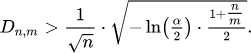
\includegraphics[width=0.4\textwidth]{pics/ks.png}
  \caption{
    Condition of a Kolmogorov-Smirnov (KS) statistic to rejects a null
    hypothesis. $D_{n,m}$ is the KS statistic, $n = m$ is the size
    of the samples, in this case, the number of HLA haplotypes ($n = m = 13$).
    $\alpha = 0.05$ is the significance level.
  }
  \label{fig:ks}
\end{figure}

%%%%%%%%%%%%%%%%%%%%%%%%%%%%%%%%%%%%%%%%%%%%%%%%%%%%%%%%%%%%%%%%%%%%%%%%%%%%%%%%
\subsection{MHC-2}
%%%%%%%%%%%%%%%%%%%%%%%%%%%%%%%%%%%%%%%%%%%%%%%%%%%%%%%%%%%%%%%%%%%%%%%%%%%%%%%%

\iffalse
	Transmembrane helices and strong MHC-II-binding peptides
	were predicted for a tuberculosis reference proteome 
	from \url{https://www.ebi.ac.uk/reference_proteomes}
	using the \verb;epitopeome; R package (\cite{epitopeome}).
	We picked the three MHC-II alleles that are most abundant 
	in the current human population, 
	which are DRB4*0101, HLA-DPA10103-DPB10402 
	\richel{
	  We decided for DPB1*0402, but there are multiple alleles matching.
	  I just picked the first one of the alleles matching, which are:
	  HLA-DPA10x-DPB10402, where x equals 103-110, 201-204, 301-303 or 401
	}
	and DQA1*0501/DQB1*0301 \richel{reference here}.
	The 5\% peptides with the lowest IC50 values were defined as binders.
	We then simply counted the number of amino acids that were present inside the
	cell, within the membrane or outside of the cell, as well as if it was part 
	of a strong MHC-II binding site, as shown in figue \ref{tab:results}.


	The \verb;epitopeome; R package (\cite{epitopeome}) binds 
	together the \verb;tmhmm; (\cite{tmhmm}) and \verb;netmhc2pan; 
	(\cite{netmhc2pan}) 
	R packages. \verb;tmhmm; provides an R interface to
	TMHMM (\cite{krogh2001predicting, sonnhammer1998hidden}), a tool
	to predict where membrane proteins' amino acids are located within the
	membrance.   
	\verb;netmhc2pan; provides an R interface to
	NetMHC2pan (\cite{jensen2018improved}), a tool
	to predict MHC-II binding to proteins.
\fi

%%%%%%%%%%%%%%%%%%%%%%%%%%%%%%%%%%%%%%%%%%%%%%%%%%%%%%%%%%%%%%%%%%%%%%%%%%%%%%%%
\subsection{Evolutionary conservation}
%%%%%%%%%%%%%%%%%%%%%%%%%%%%%%%%%%%%%%%%%%%%%%%%%%%%%%%%%%%%%%%%%%%%%%%%%%%%%%%%

\iffalse
	The evolutionary conservation of TMHs was measured from a
	DNA alignment of multiple transmembrane proteins in multitiple
	species of the mycoplasma bacterial family
	\richel{how obtained exactly? how alignment done?}.

	Using the \verb;tmhprot; R package (\cite{tmhprot}), the DNA alignment is split
	into two alignments, one for the TMH parts, another for the non-TMH
	parts. Each alignment was tested by the \verb;mcbette; 
	R package (\cite{mcbette}) to select the Bayesian inference model with
	the highest evidence (a.k.a. the marginal likelihood) using the nested
	sampling approach as described in \cite{maturana2018model},
	using the popular Bayesian phylogenetic tool 
	BEAST2 (\cite{bouckaert2014beast}) in the back-end.
	\verb;mcbette; used a set of 40 candidate inference models, 
	consisting of all combinations of 
	4 site models (JC, HKY, TN, GTR), 
	2 clock models (strict, RLN) and 
	5 tree priors (Yule, BD, CBS, CCP, CEP).

	For each alignment, the inference model with the highest evidence
	is used in a Bayesian inference. From each Bayesian posterior,
	the parameter estimates regarding mutation rates (including clock rate)
	were obtained and compared to determine which realized mutation rate is lower.
	The Markov chain Monte Carlo was set up in such a way that the effective sample
	size for the likelihood of the inference model is above the recommended value
	of 200 (\cite{bouckaert2014beast}).
\fi

%%%%%%%%%%%%%%%%%%%%%%%%%%%%%%%%%%%%%%%%%%%%%%%%%%%%%%%%%%%%%%%%%%%%%%%%%%%%%%%%
\section{Results}
%%%%%%%%%%%%%%%%%%%%%%%%%%%%%%%%%%%%%%%%%%%%%%%%%%%%%%%%%%%%%%%%%%%%%%%%%%%%%%%%

%%%%%%%%%%%%%%%%%%%%%%%%%%%%%%%%%%%%%%%%%%%%%%%%%%%%%%%%%%%%%%%%%%%%%%%%%%%%%%%%
\subsection{MHC-I}
%%%%%%%%%%%%%%%%%%%%%%%%%%%%%%%%%%%%%%%%%%%%%%%%%%%%%%%%%%%%%%%%%%%%%%%%%%%%%%%%

Figure \ref{fig:1} shows the percentages of epitopes overlapping 
with TMHs for a human and COVID-19 proteome.
The KS test to determine if these percentages are sampled from
a same distribution resulted in a p-value of \richel{unknown},
which makes us reject/accept the hypothesis that these percentages
are sampled from a same distribution. 

\begin{figure}[!htbp]
  \includegraphics[width=\textwidth]{ks/fig_1_watermarked.png}
  \caption{
    \% epitopes overlapping with transmembrane helix
    for a human and COVID-19 proteome
  }
  \label{fig:1}
\end{figure}



%%%%%%%%%%%%%%%%%%%%%%%%%%%%%%%%%%%%%%%%%%%%%%%%%%%%%%%%%%%%%%%%%%%%%%%%%%%%%%%%
\subsection{MHC-II}
%%%%%%%%%%%%%%%%%%%%%%%%%%%%%%%%%%%%%%%%%%%%%%%%%%%%%%%%%%%%%%%%%%%%%%%%%%%%%%%%

%%%%%%%%%%%%%%%%%%%%%%%%%%%%%%%%%%%%%%%%%%%%%%%%%%%%%%%%%%%%%%%%%%%%%%%%%%%%%%%%
\subsection{Evolutionary conservation}
%%%%%%%%%%%%%%%%%%%%%%%%%%%%%%%%%%%%%%%%%%%%%%%%%%%%%%%%%%%%%%%%%%%%%%%%%%%%%%%%

\iffalse
	Table \ref{tab:results} shows the location and binding strength for the
	tuberculosis proteome.

	\begin{figure}[ht]
	  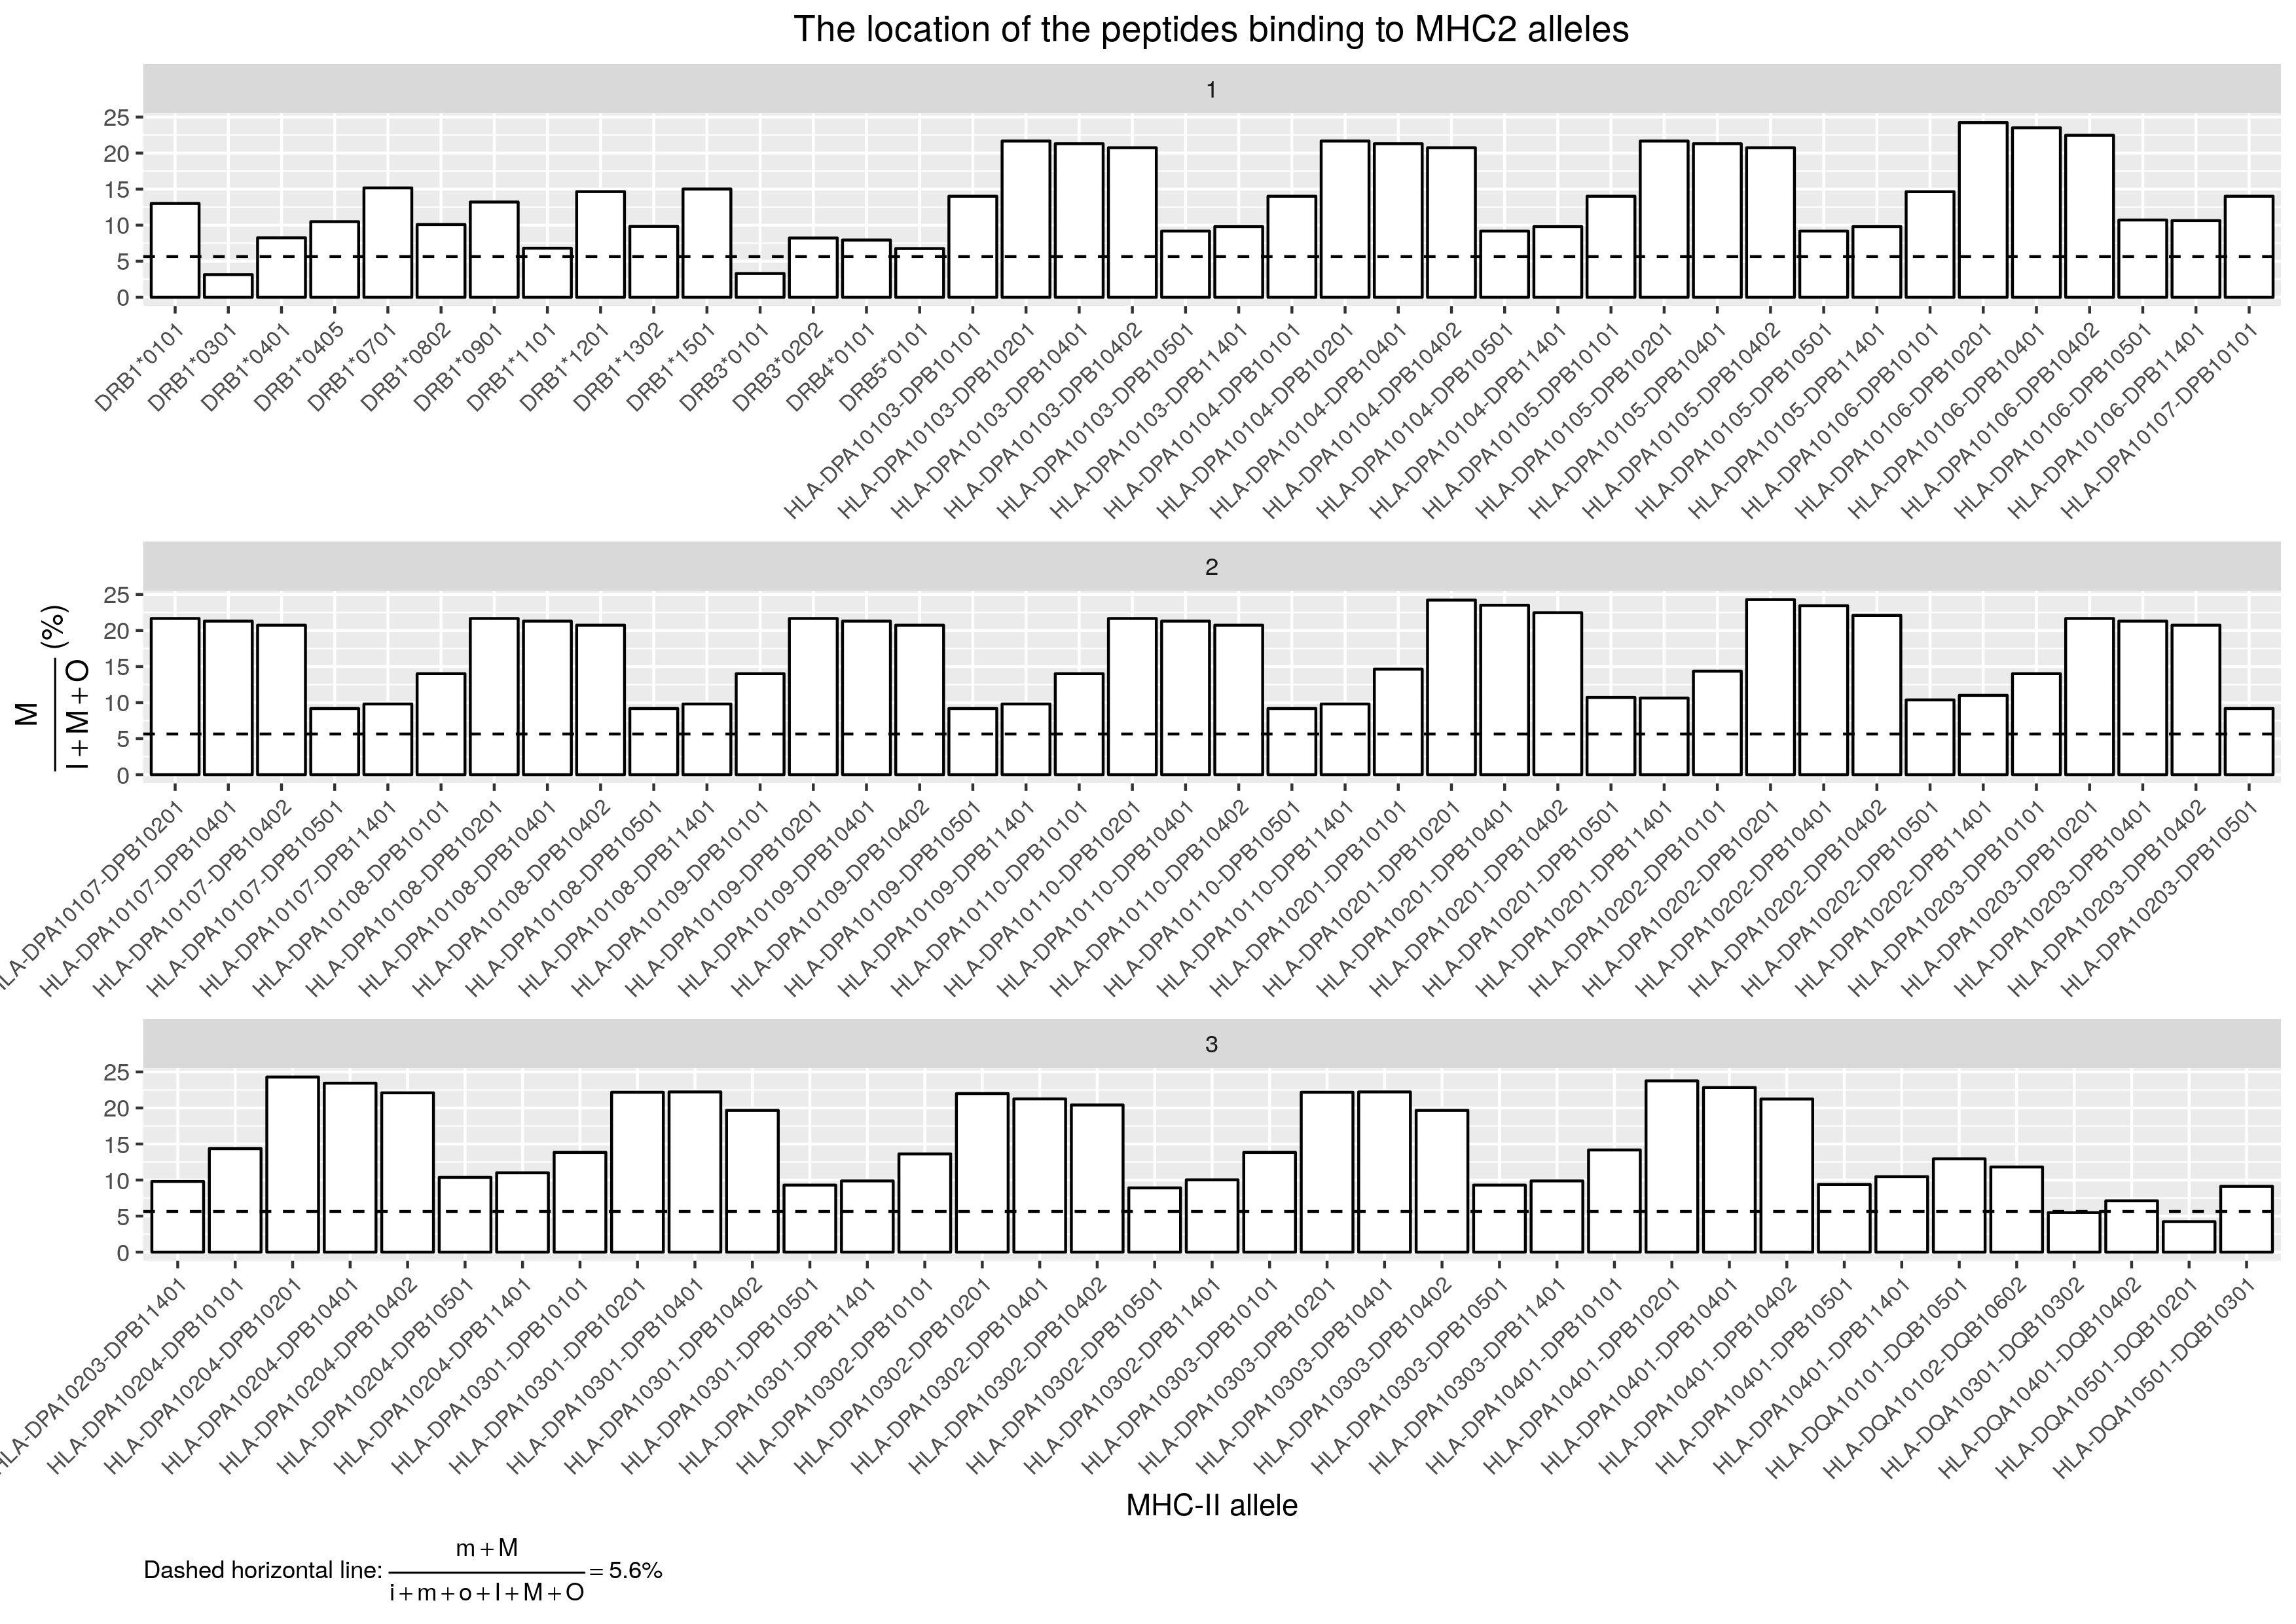
\includegraphics[width=\textwidth]{figure_1.png}
	  \label{fig:1}
	\end{figure}

	\begin{figure}[ht]
	  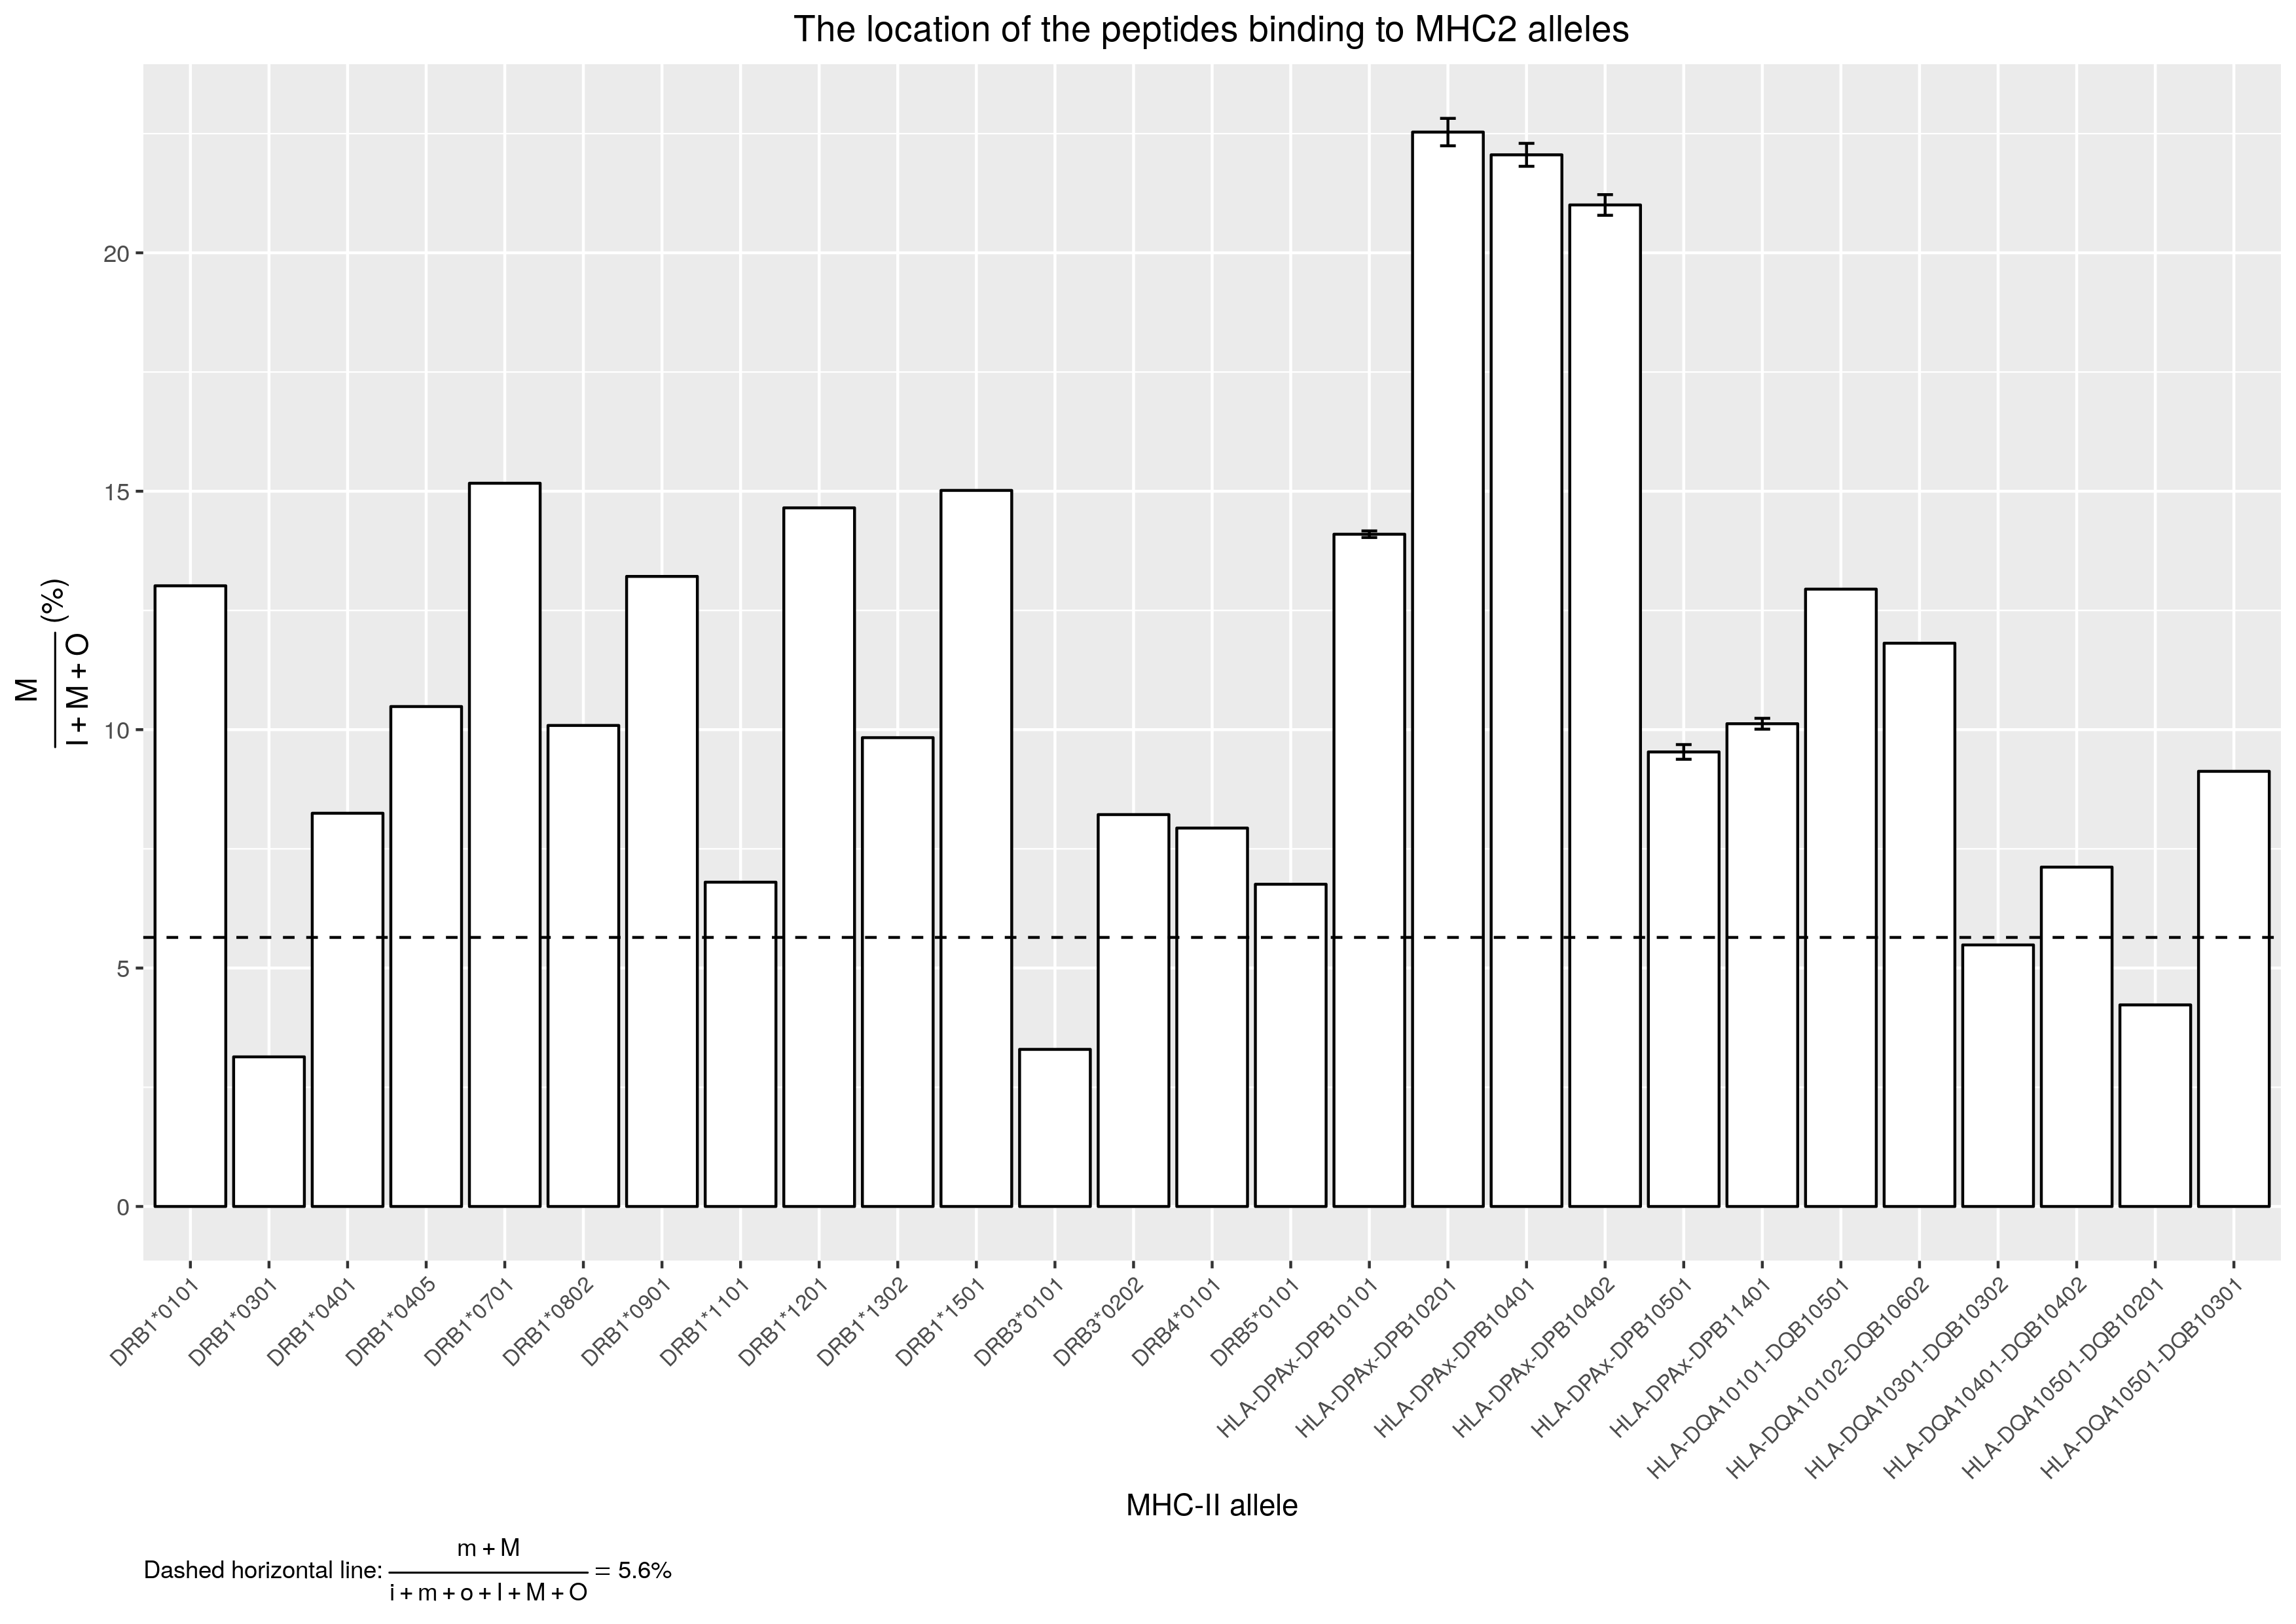
\includegraphics[width=\textwidth]{figure_1_5.png}
	  \label{fig:1_5}
	\end{figure}

	\begin{figure}[ht]
	  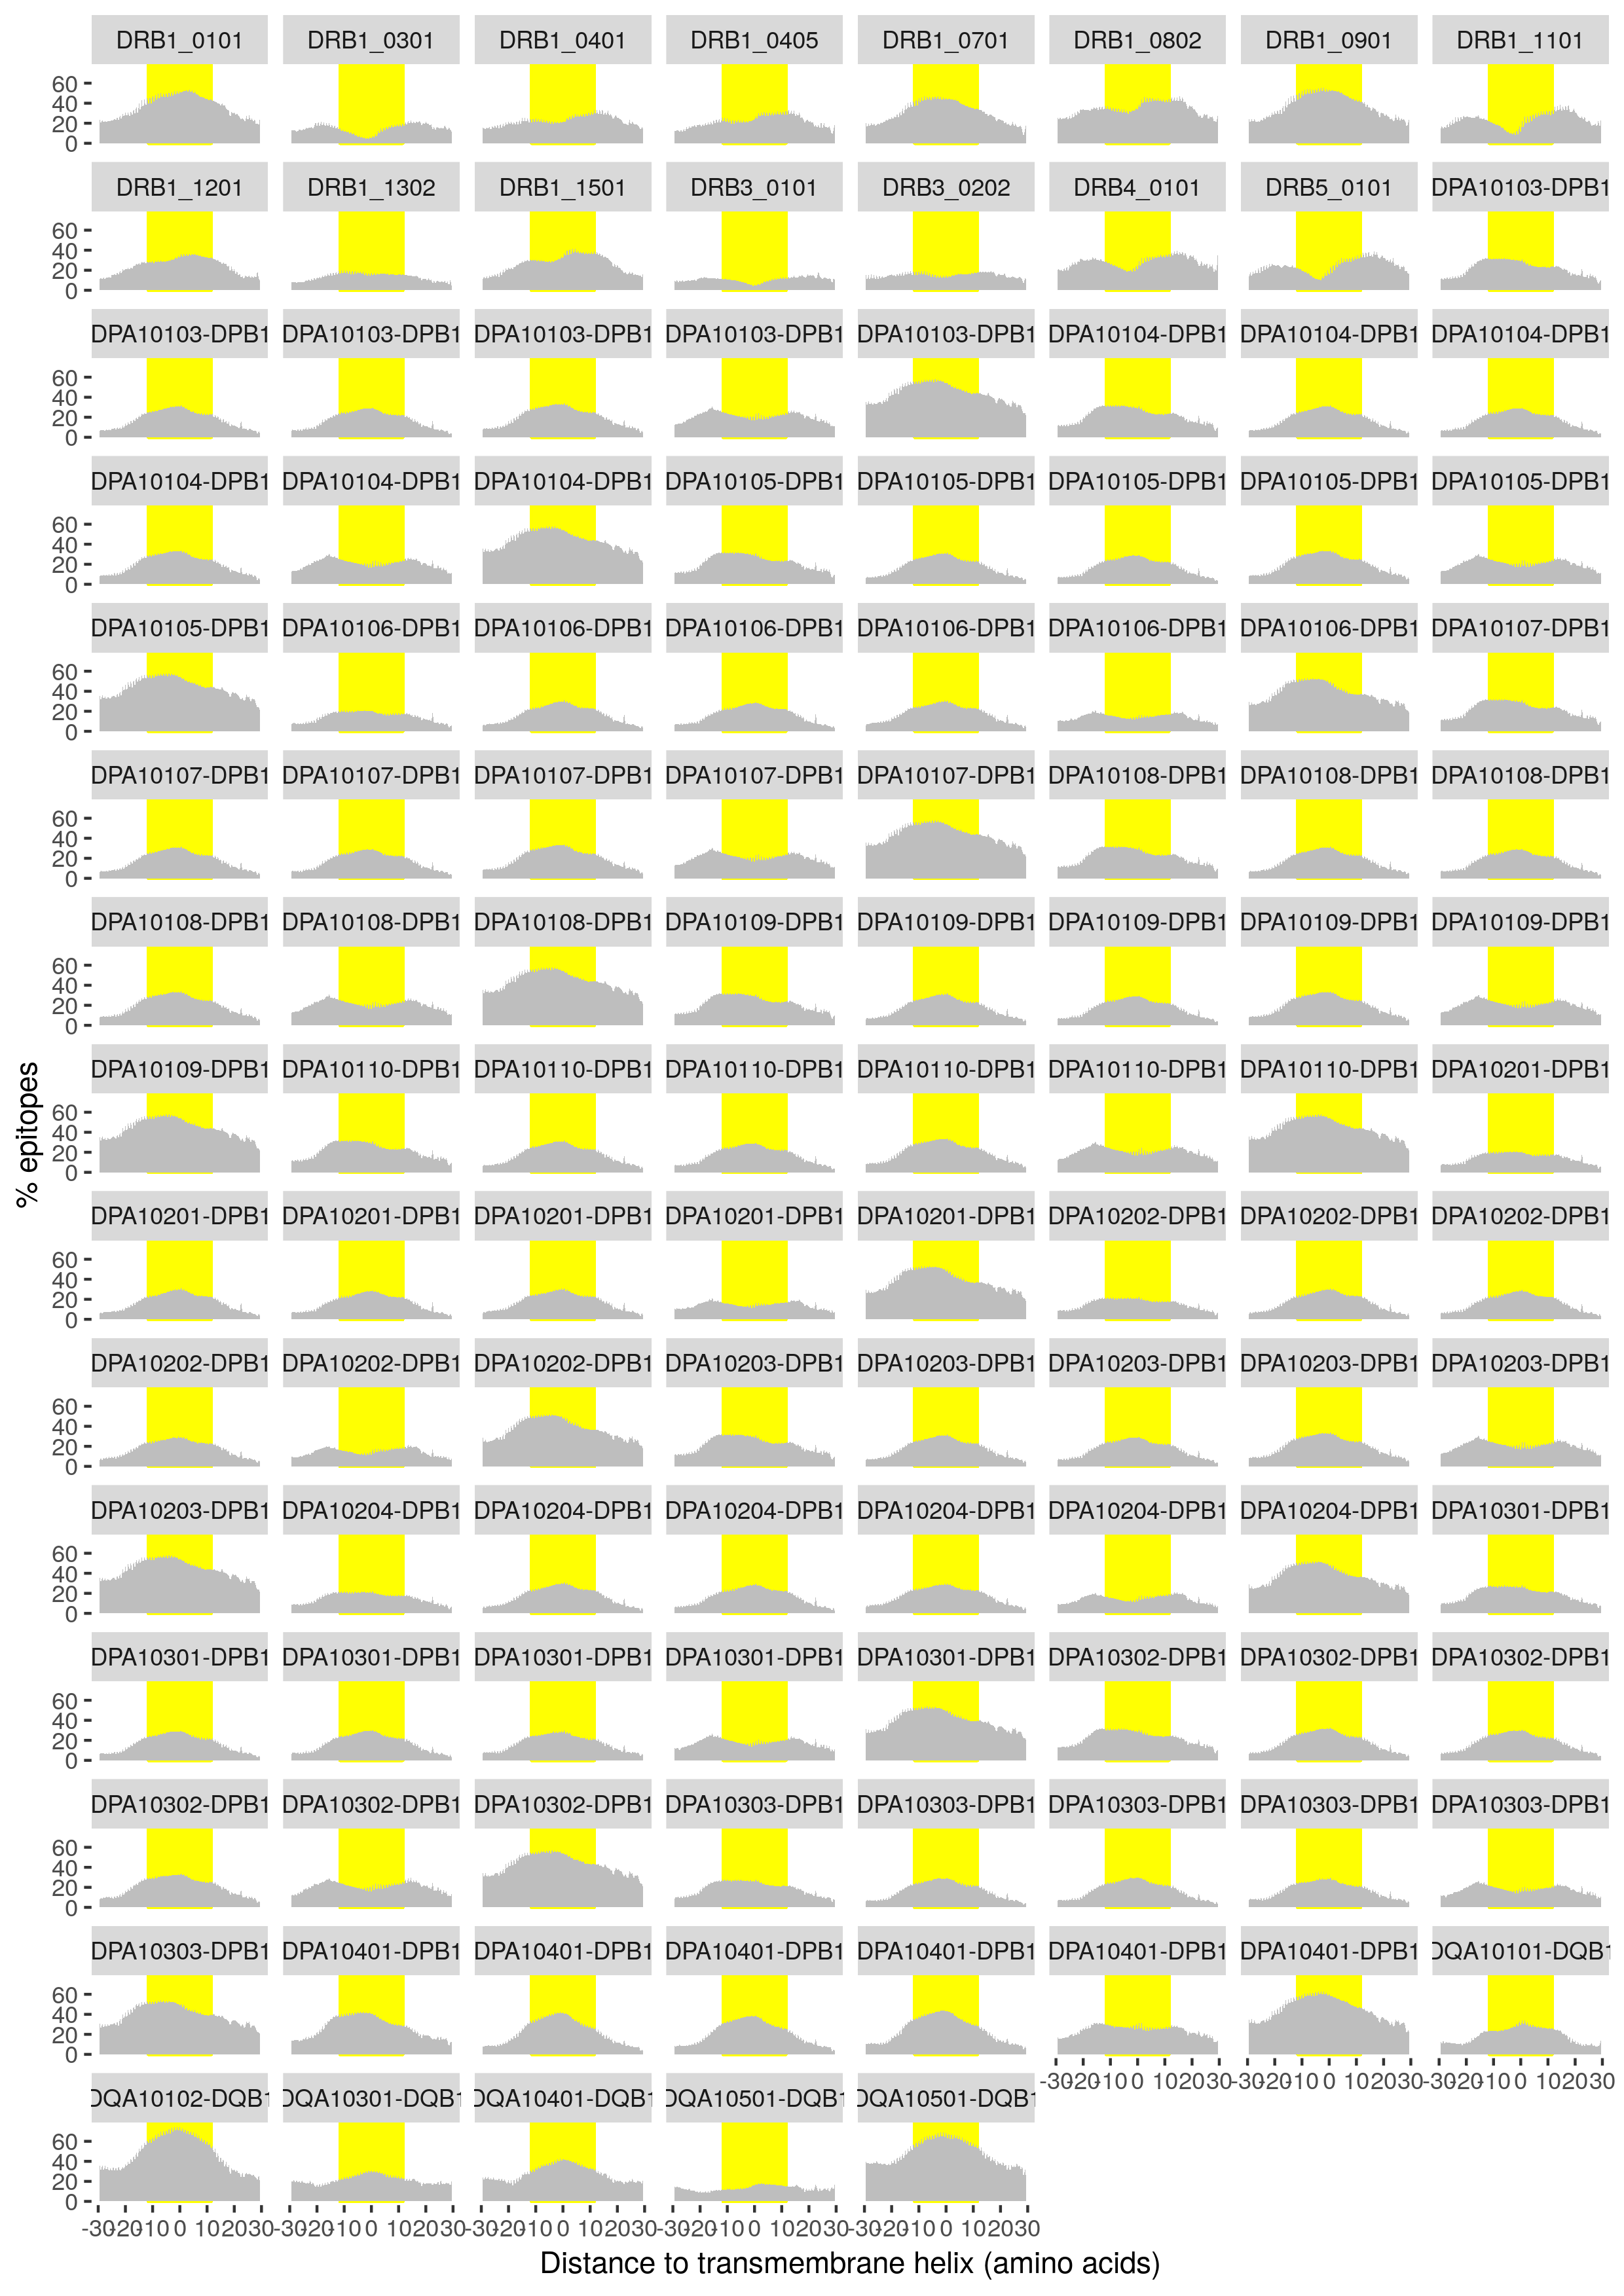
\includegraphics[width=\textwidth]{figure_3.png}
	  \label{fig:3}
	\end{figure}




	\input{table_imoimo.latex}
	% has label tab:results
	\richel{
	  I'd enjoy 
	  (1) a row with 'expected by chance', 
	  (2) using percentages instead,
	  (3) merging inside and outside
	}

	The inference model with the highest evidence in the
	TMH-only alignment was [yet unknown] and [also yet unknown]
	for the non-TMH alignment. Individual model weights are shown
	in tables \ref{tab:evidences_tmh} 
	and \ref{tab:evidences_non_tmh}.

	The Bayesian inference resulted in [a distribution of mutation rates],
	as shown in [absent figure].
	The ESSes of the Bayesian parameter estimates was above 200, exact values
	are shown in tables \ref{tab:esses_tmh} and \ref{tab:esses_non_tmh}.
\fi

%%%%%%%%%%%%%%%%%%%%%%%%%%%%%%%%%%%%%%%%%%%%%%%%%%%%%%%%%%%%%%%%%%%%%%%%%%%%%%%%
\section{Conclusion}
%%%%%%%%%%%%%%%%%%%%%%%%%%%%%%%%%%%%%%%%%%%%%%%%%%%%%%%%%%%%%%%%%%%%%%%%%%%%%%%%

We found that the percentages of epitopes overlapping 
with TMHs for a human and COVID-19 proteome are 
[similar/different]. In other words, the
epitopes that MHC-I presents are [as/not as] likely 
to be derived from TMH within either a human host and its viral pathogen.

\iffalse
	We conclude that MHC-II binds to TMH peptides with a higher/lower/equal
	probability than expected by chance. 

	We conclude that the evolutionary conservation if the TMH parts of membrane
	proteins is higher/less/equal compare to its non-TMH counterparts.
\fi

%%%%%%%%%%%%%%%%%%%%%%%%%%%%%%%%%%%%%%%%%%%%%%%%%%%%%%%%%%%%%%%%%%%%%%%%%%%%%%%%
\section{Discussion}
%%%%%%%%%%%%%%%%%%%%%%%%%%%%%%%%%%%%%%%%%%%%%%%%%%%%%%%%%%%%%%%%%%%%%%%%%%%%%%%%

We concluded that the
epitopes that MHC-I presents are [as/not as] likely 
to be derived from TMH within either a human host and its viral pathogen.
Because the full COVID-19 only has 4 TMHs \richel{check}, the percentages
of HMC-I epitopes being part of a TMH are likelier to be affected by
stochasticity. We chose to use COVID-19 regardless, as the thousands
of its time-dated genomic sequences are ideal for determining the 
evolutionary conservation of MHC-I detecting TMHs. 

\iffalse
	We compared the mutation rates between the TMH and non-TMH part of
	multiple mycoplasma species. Where we expect no variation 
	in mutation rate for every TMH amino acid,
	\richel{
	  we can test this, but unsure if that would make sense
	}
	we know that non-TMH part will have regions of different evolutionary
	conservation: functional domains, especially in protein-protein
	interactions will be strongly conserved, due to an even more constrained
	set of peptides that enable a certain function.

	\richel{
	  Note that most bacteria are opportunistic pathogens.
	  Note that most bacteria are generalists.
	  Note that most bacteria have different cell membranes (and walls), that
	  may have different functional constraints than a human cell membrane
	}
\fi

%%%%%%%%%%%%%%%%%%%%%%%%%%%%%%%%%%%%%%%%%%%%%%%%%%%%%%%%%%%%%%%%%%%%%%%%%%%%%%%%
\section{Acknowledgements}
%%%%%%%%%%%%%%%%%%%%%%%%%%%%%%%%%%%%%%%%%%%%%%%%%%%%%%%%%%%%%%%%%%%%%%%%%%%%%%%%

We thanks to Geert van den Bogaart for his wisdom.

%%%%%%%%%%%%%%%%%%%%%%%%%%%%%%%%%%%%%%%%%%%%%%%%%%%%%%%%%%%%%%%%%%%%%%%%%%%%%%%%
\section{Data Accessibility}
%%%%%%%%%%%%%%%%%%%%%%%%%%%%%%%%%%%%%%%%%%%%%%%%%%%%%%%%%%%%%%%%%%%%%%%%%%%%%%%%

All code is archived at \url{http://github.com/richelbilderbeek/someplace},
with DOI \url{https://doi.org/12.3456/zenodo.1234567}.

%%%%%%%%%%%%%%%%%%%%%%%%%%%%%%%%%%%%%%%%%%%%%%%%%%%%%%%%%%%%%%%%%%%%%%%%%%%%%%%%
\section{Authors' contributions}
%%%%%%%%%%%%%%%%%%%%%%%%%%%%%%%%%%%%%%%%%%%%%%%%%%%%%%%%%%%%%%%%%%%%%%%%%%%%%%%%

RJCB and FB conceived the idea for this research. 
RJCB wrote the code.
RJCB and FB wrote the article.

%%%%%%%%%%%%%%%%%%%%%%%%%%%%%%%%%%%%%%%%%%%%%%%%%%%%%%%%%%%%%%%%%%%%%%%%%%%%%%%%
% Bibliography
%%%%%%%%%%%%%%%%%%%%%%%%%%%%%%%%%%%%%%%%%%%%%%%%%%%%%%%%%%%%%%%%%%%%%%%%%%%%%%%%
% MEE style
\bibliographystyle{mee}
\bibliography{article}
%%%%%%%%%%%%%%%%%%%%%%%%%%%%%%%%%%%%%%%%%%%%%%%%%%%%%%%%%%%%%%%%%%%%%%%%%%%%%%%%


%%%%%%%%%%%%%%%%%%%%%%%%%%%%%%%%%%%%%%%%%%%%%%%%%%%%%%%%%%%%%%%%%%%%%%%%%%%%%%%%
\appendix
\section{Supplementary materials}
%%%%%%%%%%%%%%%%%%%%%%%%%%%%%%%%%%%%%%%%%%%%%%%%%%%%%%%%%%%%%%%%%%%%%%%%%%%%%%%%

%%%%%%%%%%%%%%%%%%%%%%%%%%%%%%%%%%%%%%%%%%%%%%%%%%%%%%%%%%%%%%%%%%%%%%%%%%%%%%%%
\subsection{Binding}
%%%%%%%%%%%%%%%%%%%%%%%%%%%%%%%%%%%%%%%%%%%%%%%%%%%%%%%%%%%%%%%%%%%%%%%%%%%%%%%%

\input{ks/table_1.latex}

\end{document}
